\label{fundamentos}

Este capítulo apresenta uma revisão dos principais conceitos relacionados ao tema deste trabalho, 
envolvendo arquiteturas orientadas a serviços com foco em modernização de sistemas legados, estando estruturado da 
seguinte forma: a Se\c c\~{a}o~\ref{arq_soa} dá uma visão geral de \acrfull{SOA}. 
A Subseção~\ref{elem_soa} descreve os componentes de um ambiente \acrshort{SOA}.
A Subse\c c\~{a}o~\ref{tec_web_services} investiga duas opções de tecnologia para implementação de \textit{Web Services}. A Subse\c c\~{a}o~\ref{justificativa_uso_rest} apresenta as justificativas para o uso 
do estilo arquitetural \acrshort{REST}. A Subse\c c\~{a}o~\ref{restricoes_rest} apresenta o conjunto de restrições de \acrshort{REST} que devem ser compreendidos para este trabalho. Por fim, na Seção~\ref{design_proj},
estuda-se duas abordagens de modelagem de domínio do negócio de um software.


\section{Service Oriented Architecture (SOA)}%
\label{arq_soa}


O termo \acrshort{SOA} foi usado pela primeira vez em 1996, quando Roy Schulte e Yeffim V. Natiz (ambos do Gartner) definiram-na como ``um estilo de 
computação de múltiplas camadas que ajudam as organizações a compartilharem as lógicas e os dados de negócios entre os sistemas computacionais''~\cite{SOA_patterns_2012}.

De forma simplificada, \acrshort{SOA} compreende uma arquitetura corporativa onde os serviços são criados, reutilizados e compartilhados entre os vários sistemas de uma 
organização em um sistema distribuído de modo que as funcionalidades possam estar disponíveis a todos os interessados que estejam autorizados a usá-las~\cite{S05_Lewis:2005, S04_IntLgSw:2006}.

Serviços são componentes de software que encapsulam conceitos de negócios de alto nível, composto basicamente por três elementos: a interface, o contrato e a implementação do serviço. A interface define como o fornecedor do serviço viabiliza as requisições dos clientes; o contrato do serviço descreve o serviço (funcionalidade, parâmetros, restrições entre outros atributos); e a implementação é o código do serviço em si~\cite{krafzig2004service}. 

Nesse contexto, como observado em~\cite{SOAAprocIntegr:2007}, essa arquitetura corporativa tem sido amplamente utilizada nas organizações em projetos envolvendo a modernização dos sistemas legados, onde os serviços representam os ativos principais com interfaces bem definidas, que podem ser decompostas em módulos interoperáveis possuindo algumas características importantes descritas a seguir~\cite{fielding2000architectural,SOA_patterns_2012}:

\begin{description}
\item[Valor agregado.] Refere-se à capacidade dos serviços de fornecerem 
valor agregado ao negócio da organização, a qual não recomenda-se que 
funcionalidades de baixo nível sejam expostas como serviços. Para exemplificar, não faz sentido o \acrshort{CPD} disponibilizar serviços como bibliotecas de funções (como tratamento de texto, data e hora, etc) já que não vai agregar valor ao negócio (e possivelmente ocasionar \textit{overhead} na rede ~\cite{fielding2000architectural}).

\item[Visibilidade.] Capacidade dos serviços de serem encontrados pelos 
interessados e que suas interfaces sejam bem compreendidas pelo invocador. Neste trabalho, a visibilidade será implementada por meio de um catálogo de serviços que poderá ser consultado em um portal.

\item[Autocontido.] Os serviços não devem depender de informações do contexto
de outros serviços e também não devem armazenar estados entre as requisições de serviços.

\item[Baixo acoplamento.] É um design de arquitetura dos sistemas distribuídos que 
determina que diferentes partes e funcionalidades de um sistema sejam independentes umas das outras. 
Assim, alterações em uma determinada parte do sistema não trará consequências para o resto do sistema, 
trazendo benefícios como escalabilidade, flexibilidade e tolerância a falhas.
\end{description}

Com base nas características apresentadas, pode-se inferir que em um ambiente \acrshort{SOA}, os sistemas críticos (possivelmente grandes e complexos) deveriam ser substituídos por sistemas mais simples a partir da composição dos serviços disponíveis em um ambiente distribuído. Essa estratégia representa uma possibilidade para a modernização do \acrfull{SIGRA} da \acrlong{UnB}. 

Dado os benefícios percebidos na literatura, \acrshort{SOA} tem potencial para prover mais flexibilidade na modernização dos sistemas legados, haja vista os benefícios com reuso e compartilhamento das funcionalidades que podem ser obtidos. Contudo, no contexto da \acrshort{UnB}, o uso de uma abordagem orientada a serviço ainda precisa ser investigada, pois como afirmam os autores ~\cite{fielding2000architectural,ModelDriApproRest:2014,SOAIntBlueprint:2010,SOA_patterns_2012}, há alguns \textit{trade-offs} a considerar, entre eles, a maior complexidade dos sistemas distribuídos; a preocupação com a segurança e acesso aos serviços, o \textit{overhead} ocasionado na rede com a troca de mensagens; e a necessidade das equipes de TI dominarem algumas tecnologias talvez não habituadas.


\subsection{Componentes de um Ambiente SOA}\label{elem_soa}%

Um ambiente \acrshort{SOA} abrange a interação de três componentes: o provedor do serviço (\textit{Service Provider}), o consumidor (\textit{Service Consumer}) e o catálogo de serviços (\textit{Service Broker})~\cite{SOAIntBlueprint:2010,SOA_patterns_2012}. A interação entre esses elementos é conhecida como ``\textit{find-bind-execute paradigm}''~\cite{papazoglou2003service}, que significa paradigma ``procura-consolida-executa''. De forma resumida, 
os provedores (que são os fornecedores dos serviços) devem consolidar as informações sobre os serviços 
no catálogo de serviços (um repositório central para os serviços) com a descrição desses serviços. Com base nas informações armazenadas nesse catálogo, os consumidores (que são os clientes) podem identificar e solicitar a execução dos serviços requeridos junto ao provedor, conforme ilustra a Figura~\ref{fig:soa}.

\begin{enumerate}[(a)]

\item Provedor do Serviço. Na perspectiva do negócio, corresponde ao dono do serviço ou o fornecedor do serviço. Em uma perspectiva arquitetural, é a plataforma onde os \textit{hosts} (usuários dos serviços) acessam os serviços oferecidos. O provedor de serviços disponibiliza acesso aos serviços e a especificação desses serviços são publicadas no registro de serviços. Essa publicação permite que os clientes localizem os serviços e requisitem sua execução ao provedor.

\item Consumidor do Serviço. São os clientes que requisitam serviços. Note que, o consumidor do serviço por ser uma pessoa, uma aplicação ou mesmo outro serviço;

\item Catálogo de Serviços. É a localização central dos serviços (como  um repositório) onde o provedor pode publicar tais serviços e o consumidor pode encontrá-los. 

\end{enumerate}


\begin{figure}[!hbt]
\centering
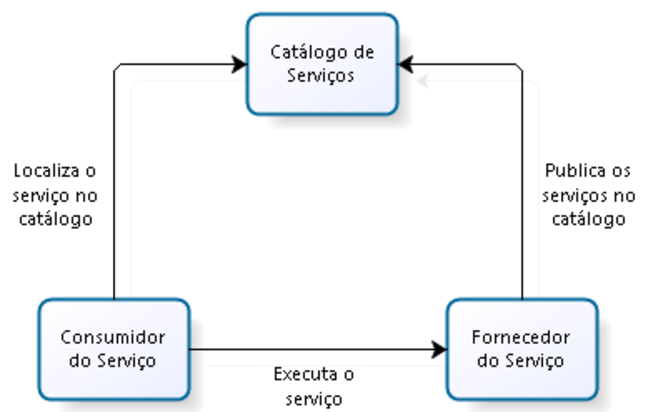
\includegraphics[scale=0.80]{img/fundamentos/soa.pdf}
\caption{Relacionamentos entre os elementos de uma arquitetura \acrshort{SOA}.}
\label{fig:soa}
\end{figure}




\subsection{Web Services \acrshort{SOAP} e REST}\label{tec_web_services}%

Destacam-se atualmente duas tecnologias para a implementação 
de um ambiente \acrshort{SOA}, os \textit{Web Services} \acrshort{SOAP} e  \acrshort{REST}. Ambos são muito utilizados (e até mesmo combinados) para invocação de serviços de negócios em um sistema distribuído~\cite{SOAIntBlueprint:2010,SOA_patterns_2012}. O transporte de dados desses serviços é realizado tipicamente pelos protocolos \acrfull{HTTP} ou \acrfull{HTTPS} para conexões seguras. 

Os \textit{Web Services} \acrshort{SOAP}, acrônimo de \acrlong{SOAP} representam um conjunto de tecnologias e padrões da indústria definidas pela \acrfull{W3C} com um suporte tecnológico bastante maduro por parte dos fornecedores de tecnologia que as suportam~\cite{S04_IntLgSw:2006}. Este tipo de \textit{Web Service} é baseado na linguagem \acrfull{XML} para a especificação da estrutura e o formato das mensagens, impondo restrições no formato das mensagens (funcionando como um contrato de serviço). A linguagem \acrshort{XML} consiste basicamente em uma linguagem de marcação extensível, quer permite especificar as mensagens de forma simples e legível por meio de \textit{tags} personalizadas~\cite{S04_IntLgSw:2006}. Por exemplo, em \acrshort{SOAP}, tanto a descrição dos serviços como a requisição e a resposta de uma invocação a um serviço são mensagens no formato \acrshort{XML}. Usa-se a linguagem \acrshort{WSDL} para descrever a estrutura das mensagens \acrshort{SOAP} e as ações possíveis em um \textit{endpoint} (\acrshort{URL} onde o serviço pode ser acessado pela aplicação). Assim, o \acrshort{WSDL} nada mais é do que um documento em formato \acrshort{XML} descrevendo o serviço oferecido, como acessá-lo, e quais as operações e os métodos disponíveis na especificação do serviço~\cite{SOAIntBlueprint:2010}. 



Os \textit{Web Services} \acrshort{REST}, acrônimo de \acrlong{REST} representam outro tipo de serviço que está sendo adotado pelas organizações (substituindo ou complementando os \textit{Web Services} \acrshort{SOAP}). De acordo com Roy Fielding~\cite{fielding2000architectural}, \acrshort{REST} é um estilo arquitetural baseado no protocolo de hipermídia \acrshort{HTTP}, sendo introduzido para implementar \textit{Web Services} fracamente acoplados. O \acrfull{JSON} é um formato para intercâmbio de dados  (baseado em um subconjunto da notação de objetos da linguagem Javascript~\cite{bray2014javascript}) utilizado preferencialmente neste tipo de serviço como uma alternativa mais simples
e leve ao \acrshort{XML}~\cite{richardson2008restful}.
\acrshort{REST} baseia-se em recursos e verbos~\cite{fielding1999rfc}. Cada recurso pode ser referenciado através de sua \acrshort{URI} (por exemplo, \texttt{http://sistemas.unb.br/alunos/100} obtém o recurso aluno cuja a identificação é 100). As ações de um recurso são providas pelos verbos do protocolo \acrshort{HTTP}, que compreendem os métodos \textit{GET} para obter a representação de um recurso; \textit{POST} para criar novos recursos; \textit{PUT} para modificar um recurso existente; \textit{DELETE} para excluir um recurso existente. Também podem ser usados os m\'{e}todos \textit{HEADER}, para recuperar os metadados de uma representação do recurso e \textit{OPTIONS} para obter a descrição ou a documentação sobre o recurso desejado. 

Os \textit{Web Services} facilitam a interoperabilidade entre aplicações heterogêneas. Nesta seção, foram investigadas duas opções de tecnologia para implementar uma abordagem \acrshort{SOA}, embora existam outras alternativas disponíveis no mercado. Salienta-se que ambas tecnologias (\acrshort{SOAP} e \acrshort{REST}) são perfeitamente viáveis para o propósito do trabalho. No entanto, optou-se por experimentar o \acrshort{REST}, uma abordagem emergente que tem tido cada vez mais aceitação na indústria devido
a sua flexibilidade e porque o CPD/UnB está interessado em utilizá-lo. No restante deste capítulo será apresentado em mais detalhes a abordagem \acrshort{REST} e as restrições deste estilo arquitetural que se fazem importantes para o trabalho de dissertação.




\subsection{Justificativa para o Uso de REST}\label{justificativa_uso_rest}%

Os \textit{Web Services} impõem uma camada de abstração que permitem aos componentes do tipo cliente, solicitar serviços aos componentes do tipo servidor~\cite{richardson2008restful}. No entanto, essas abstrações 
frequentemente causam alguma lentidão (\textit{overhead}), comprometendo o desempenho 
das aplicações, como observado em~\cite{fielding2000architectural}. Isso é mais evidente em \acrshort{SOAP} devido ao tamanho das mensagens, já que tais mensagens são descritas na linguagem \acrshort{WSDL} e envelopadas pelo protocolo \acrshort{SOAP}, ambos no formato \acrshort{XML}~\cite{SOAIntBlueprint:2010,richardson2008restful}.

\acrshort{REST} representa uma alternativa ao \acrshort{SOAP}, pois aceita o uso de \acrshort{JSON} em vez do formato \acrshort{XML} para a especificação das mensagens~\cite{fielding2000architectural,kalin2013java}. 
Segundo~\cite{ModelDriApproRest:2014}, uma das suas principais vantagens consiste na facilidade no desenvolvimento, o aproveitamento da infraestrutura web existente e um esforço de aprendizado menor. Daí que, como este trabalho tem como foco a modernização de sistemas legados, através de uma abordagem orientada a serviço, quer se evitar que as aplicações tenham que lidar com vários protocolos (caso fosse escolhido o tipo de \textit{Web Service} \acrshort{SOAP}). Sem dúvida, o estilo arquitetural \acrshort{REST} pode ser mais facilmente adotado no \acrshort{CPD}/\acrshort{UnB}, pois os sistemas legados precisam apenas ter condições de fazer requisições \acrshort{HTTP}/\acrshort{HTTPS} aos serviços disponíveis e manipular o formato de dados \acrshort{JSON}. 

Por outro lado, \textit{Web Services} \acrshort{SOAP} apresentam algumas vantagens sobre \acrshort{REST}, conforme cita o autor~\cite{kalin2013java}: a) da perspectiva do desenvolvedor, possuem um apelo a contrato de serviços; b) a linguagem \acrshort{WSDL} usada neste tipo de serviço, permite descrever o layout das mensagens, o que de certa forma, facilita a integração dos sistemas, permitindo gerar automaticamente a implementação do cliente do \textit{Web Service} de forma padronizada; e c) o protocolo \acrshort{SOAP} compreende um método de transporte genérico, podendo usar qualquer meio de transporte para enviar a requisição (não somente \acrshort{HTTP}/\acrshort{HTTPS}). \acrshort{REST} é mais fácil de entender e acessível, porém faltam padrões e a tecnologia é considerada apenas um estilo arquitetural~\cite{fielding2000architectural}. Em contrapartida, \acrshort{SOAP} é um padrão da indústria, com protocolos bem definidos e um conjunto de regras bem estabelecidas.

Na abordagem proposta neste trabalho, um dos requisitos definidos foi o uso de um catálogo de serviço (em formato \acrshort{JSON}) para catalogar os serviços disponíveis. Espera-se que deficiências de \acrshort{REST} quanto a ausência de um formato para especificação dos serviços sejam suplantadas com uma certa flexibilidade. Não obstante, os \textit{Web Services} \acrshort{REST} já foram utilizados no \acrshort{CPD}, na implementação de um serviço para enviar dados requeridos para o \acrfull{UnBDoc} em ASP a partir do sistema \acrshort{SIEX} em Java. Essa experiência mostrou-se positiva, razão pela qual os membros da \acrfull{SSI} querem experimentar \textit{Web Services} \acrshort{REST} em uma abordagem de modernização orientada a serviços. 

Contudo, para que \acrshort{REST} possa ser utilizada no CPD/UnB de maneira correta, devem ser observados um conjunto de restrições de arquitetura, conforme afirma~\cite{fielding2000architectural}. Esse conjunto de restrições 
serão apresentados na Subseção~\ref{restricoes_rest}.



\subsection{As Restrições REST} \label{restricoes_rest}%

Para o desenvolvimento de sistemas orientado a serviços com \acrshort{REST}, existe um conjunto de restrições específicas para auxiliar o desenho das aplicações~\cite{fielding2000architectural}. Quando tais restrições são seguidas, os sistemas denominam-se \textit{RESTful}. Note que, como
sugere~\cite{flanders2008restful, RestApiDesign:2011}, as restrições de arquitetura \acrshort{REST} 
são mais do que um guia com regras e, quando aplicadas, 
torna-se possível explorar os benefícios da \textit{Web} em seu benefício.
Em resumo, as cinco restrições do estilo arquitetural \acrshort{REST} são descritas a seguir:


\subsubsection{Cliente-Servidor} 

A restrição Cliente-Servidor demanda 
a separação dos componentes cliente e servidor e estabelece uma arquitetura em camadas. 
Segundo~\cite{fielding2000architectural}, o princípio que norteia 
esta restrição é a separação das responsabilidades entre os componentes para que 
possam evoluir separadamente. Entre os benefícios disto, de 
acordo com~\cite{ModelDriApproRest:2014}, está a maximização da portabilidade 
ao permitir múltiplas interfaces com o usuário entre diferentes plataformas 
e o aumento da escalabilidade ao simplificar os componentes de servidor.

\subsubsection{Stateless} 

Esta restrição estabelece que a interação entre 
o cliente e o servidor não deve manter estados entre as comunicações. 
Assim, as requisições que o cliente envia ao servidor precisam conter 
toda a informação para descrever a solicitação, uma vez que no lado do servidor, 
não vai existir qualquer tipo de armazenamento de sessão. 

Entre os benefícios desta restrição está a escalabilidade 
do servidor, pois não há recursos alocados entre as requisições, permitindo 
liberar rapidamente os recursos após seu uso e a visibilidade, pois o servidor 
somente processa as requisições sem se preocupar com a natureza integral
do pedido~\cite{ModelDriApproRest:2014, krafzig2004service}. 

No entanto, existem alguns \textit{trade-offs}, por exemplo, a performance da 
rede pode diminuir com o aumento dos dados repetitivos vindo nas requisições pela ausência 
de estado no servidor~\cite{fielding2000architectural}. 

Embora os sistemas \textit{Web} da \acrshort{UnB} não sejam RESTFul, como comparação, verificou-se 
o emprego de uma abordagem oposta a esta restrição, chamada \textit{stateful}. Nesse caso, 
os sistemas \textit{Web} da Instituição fazem uso de sessão, que mantêm os dados do cliente na memória do 
servidor de aplicação. Como consequência, em ocasiões de muitos acessos aos sistemas, 
como nos eventos de extensão da Universidade ou no início das aulas, alguns sistemas tornam-se 
instáveis, como é o caso dos sistemas \acrfull{SISRU} e o \acrfull{SIEX}. Isso é devido aos problemas de 
escalabilidade nos servidores de aplicação identificados pelos técnicos do \acrshort{CPD} juntamente com uma 
consultoria externa contratada pelo \acrshort{CPD} em 2013.


\subsubsection{Cache} 

A restrição de \textit{cache} impõem que a resposta de uma solicitação de serviço seja 
implicitamente ou explicitamente rotulada como \textit{cacheable} (que faz uso de \textit{cache}) ou \textit{não cacheable} 
(não está sujeito ao \textit{cache}). De acordo com~\cite{ModelDriApproRest:2014}, mecanismos de \textit{cache} podem ser colocados em vários locais 
ente o servidor e o cliente. Além disso, o protocolo \acrshort{HTTP} também pode ser utilizado através dos campos do cabeçalho 
para controle do \textit{cache} das mensagens. 

O maior benefício do uso desta restrição, 
na visão de~\cite{fielding2000architectural, kalin2013java, richardson2008restful}, é o aumento do desempenho com a 
redução de chamadas ao serviço na rede. Outro benefício observado pelo autor é que eles podem eliminar parcialmente ou 
completamente algumas interações entre o cliente e o servidor, melhorando a eficiência das aplicações e a escalabilidade do servidor. 
Um \textit{trade-off} é a perca da confiabilidade, pois os dados contidos no \textit{cache} podem estar defasados em relação aos 
dados obtidos diretamente do servidor. Em razão deste \textit{trade-off}, essa restrição não será utilizada na arquitetura proposta neste trabalho.


\subsubsection{Interface Uniforme} 

Interface Uniforme impõem uma restrição na interface de troca de mensagens
entre o cliente e o servidor, 
a partir de um conjunto predefinido de 
operações, sendo 
esta restrição obtida com o uso dos verbos \acrshort{HTTP} 
com suas respectivas semânticas
~\cite{fielding1999rfc, flanders2008restful, ModelDriApproRest:2014, RestApiDesign:2011}. 

Segundo~\cite{fielding2000architectural, flanders2008restful}, 
esta restrição enfatiza o uso de uma interface uniforme entre os componentes, 
simplificando a arquitetura e melhorando a visibilidade das interações. Contudo, isso pode diminuir a eficiência das aplicações, 
pois os dados são enviados em um formato padrão, em vez de um formato específico utilizado pelas aplicações.

Para que seja possível obter uma interface uniforme, \acrshort{REST} 
define 4 restrições de interface: Identificação dos recursos, 
representação de recursos, mensagem auto descritivas e utilização 
de hipermídia para o estado da aplicação. A identificação de recursos 
estabelece que os recursos devem ser identificados. Esta restrição é 
implementada pelo \acrshort{HTTP} através da \acrshort{URI} 
do recurso que representa 
uma sequência de caracteres para localizar tal recurso físico ou abstrato~\cite{berners2012rfc}.
A representação de recursos 
diferencia o recurso de sua representação, permitindo múltiplos formatos de dados 
para um mesmo recurso, como o JSON, o \acrshort{XML} 
ou apenas texto puro~\cite{fielding1999rfc}. Para implementar esta restrição, 
REST baseia-se no \acrfull{MIME} das mensagens que são definidas no 
cabeçalho da requisição do serviço. Desta forma, o \textit{payload} (corpo das mensagens) contêm a representação do 
recurso pré-acordado entre o cliente e o servidor na solicitação da mensagem~\cite{ModelDriApproRest:2014}.
Mensagens auto descritivas requerem que as mensagens contenham toda a informação sobre o recurso para descrever a sua 
representação. Assim, as mensagens devem informar os metadados no cabeçalho para indicar como o seu conteúdo 
será tratado~\cite{fielding2000architectural}. Por fim, na restrição de utilização de hipermídia para estado da aplicação (HATEOAS), 
os recursos solicitados pelas aplicações devem possuir \textit{hiperlinks} para possibilitar a navegação entre os recursos 
relacionados~\cite{RestApiDesign:2011}. A razão disso é que o servidor não armazena estado de sessão, sendo responsabilidade do 
desenvolvedor da aplicação criar as representações adequadamente~\cite{ModelDriApproRest:2014}. Contudo, 
conforme salienta~\cite{ModelDriApproRest:2014}, esta restrição não é muito utilizada por ser um conceito novo entre os desenvolvedores.


\subsubsection{Sistema em camadas}

Essa restrição tem a finalidade de dividir o sistema em camadas para que os componentes participantes 
somente interajam com o componente adjacente. Um dos benefícios desta restrição é promover a independência entre as 
camadas e reduzir a complexidade dos sistemas. Outro benefício importante desta restrição é encapsular os serviços 
legados~\cite{fielding2000architectural}. Como \textit{trade-off}, existe uma possível redução do desempenho do sistema por 
causa do \textit{overhead} da inclusão de camadas~\cite{ModelDriApproRest:2014}.


\subsubsection{Code-On-Demand}

Esta é uma restrição opcional. Permite que as funcionalidades dos clientes sejam estendidas 
e simplificadas com o \textit{download} e execução de códigos no lado do 
cliente~\cite{fielding2000architectural}.



\section{Modelagem de Domínio do Negócio}%
\label{design_proj}

A fim de modelar um sistema, 
a literatura descreve diversos 
padrões de design de software, 
tais como a utilização de
uma arquitetura em 
camadas contendo 
artefatos especificamente projetados 
para um determinado
interesse~\cite{clements2002documenting, OORP2013, evans2004domain, fowler2002patterns, 
SOAIntBlueprint:2010, panda2007ejb, stal2006using}. 
Em~\cite{panda2007ejb}, por exemplo,
os autores abordam uma arquitetura de quatro 
camadas que permite a separação das responsabilidades entre 
as camadas e favorece a educação de novos desenvolvedores quanto a arquitetura, o planejamento do desenvolvimento incremental, o planejamento das tarefas e a definição dos prazos, entre outros.

Entretanto, alguns autores acreditam~\cite{S3_Bisbal:1999,evans2004domain,fowler2002patterns,stal2006using}, que o maior desafio está, na maioria das vezes, na complexidade para entender e modelar o domínio de negócio
com o qual a aplicação deve lidar e não na arquitetura em si do software, razão pela qual a separação em camadas possivelmente não é o suficiente. 

Para lidar com esses desafios, há alguns padrões de design identificados 
na literatura que objetivam organizar a lógica negocial. São eles: o \acrfull{DDD} e o \textit{Transaction Script}. 
Esses padrões focam-se nos aspectos de modelagem da aplicação, para que o software construído reflita adequadamente as necessidades que deverão ser contempladas para o usuário final. 

O padrão \acrshort{DDD} organiza a lógica de
domínio do negócio de um sistema em um modelo de objetos ricos, sendo indicado quando
há muita complexidade~\cite{evans2004domain, stal2006using}. Por outro lado, existem situações, nas quais um modelo de domínio rico não seria tão indicado, como na criação de cadastros simples, que não possui muita regra de negócio, por exemplo. Nessas situações, o padrão \textit{Transaction Script} poderia ser utilizado~\cite{evans2004domain}.

O padrão \textit{Transaction Script} organiza a lógica negocial do sistema em um conjunto de métodos que lidam com as requisições desde a camada de apresentação até a camada de persistência. 
O uso de \textit{Transaction Script} é bem conhecido pelos desenvolvedores da \acrfull{SSI}, pois alguns sistemas da \acrshort{UnB} que foram migrados para Java utilizam este padrão, como é o caso do \acrfull{SITAB}, do \acrfull{SITRAN}, do \acrfull{SIMAR} e do \acrfull{SIEX}. 
